






% =========----------	[ Space left here for distraction free mode] ----------==========%









\subsection{Analysis 6: Enjoyment Rating}

	The purpose of both VR and music is primarily to entertain. If users do not enjoy what they are experiencing then the cause should be addressed. For this purpose participants were asked to rate on a scale of 1-10 how much they felt they enjoyed the experience. Figure~\ref{image:enjoyment} shows the line of best fit for average enjoyment score against average spatial attribute score for each microphone for both viewing position A and B.
	
	Both graphs show a strong positive correlation between the scores for spatial attributes and enjoyment ratings with a correlation coefficient $r = 0.81$ and $r = 0.96$ for viewing position A and B respectively.

	\textbf{Conclusion} \\
	This suggests that when provided with higher quality spatial audio for an experience such as the one presented, viewers are more likely to enjoy the experience. It is important to address that this VR experience differs from the currently most popular form of VR experience available which is gaming. VR games offer the possibility of movement and interaction which may distract users from the quality of spatial audio. However, in an experience such as the one presented in this paper, where the focus of the experience is listening to music and lateral movement is not an option, the users focus is not taken away from the spatial audio quality. It is therefore important for listening to music in VR that the spatial audio quality is high to ensure the listening experience is enjoyed.



	\begin{figure}
		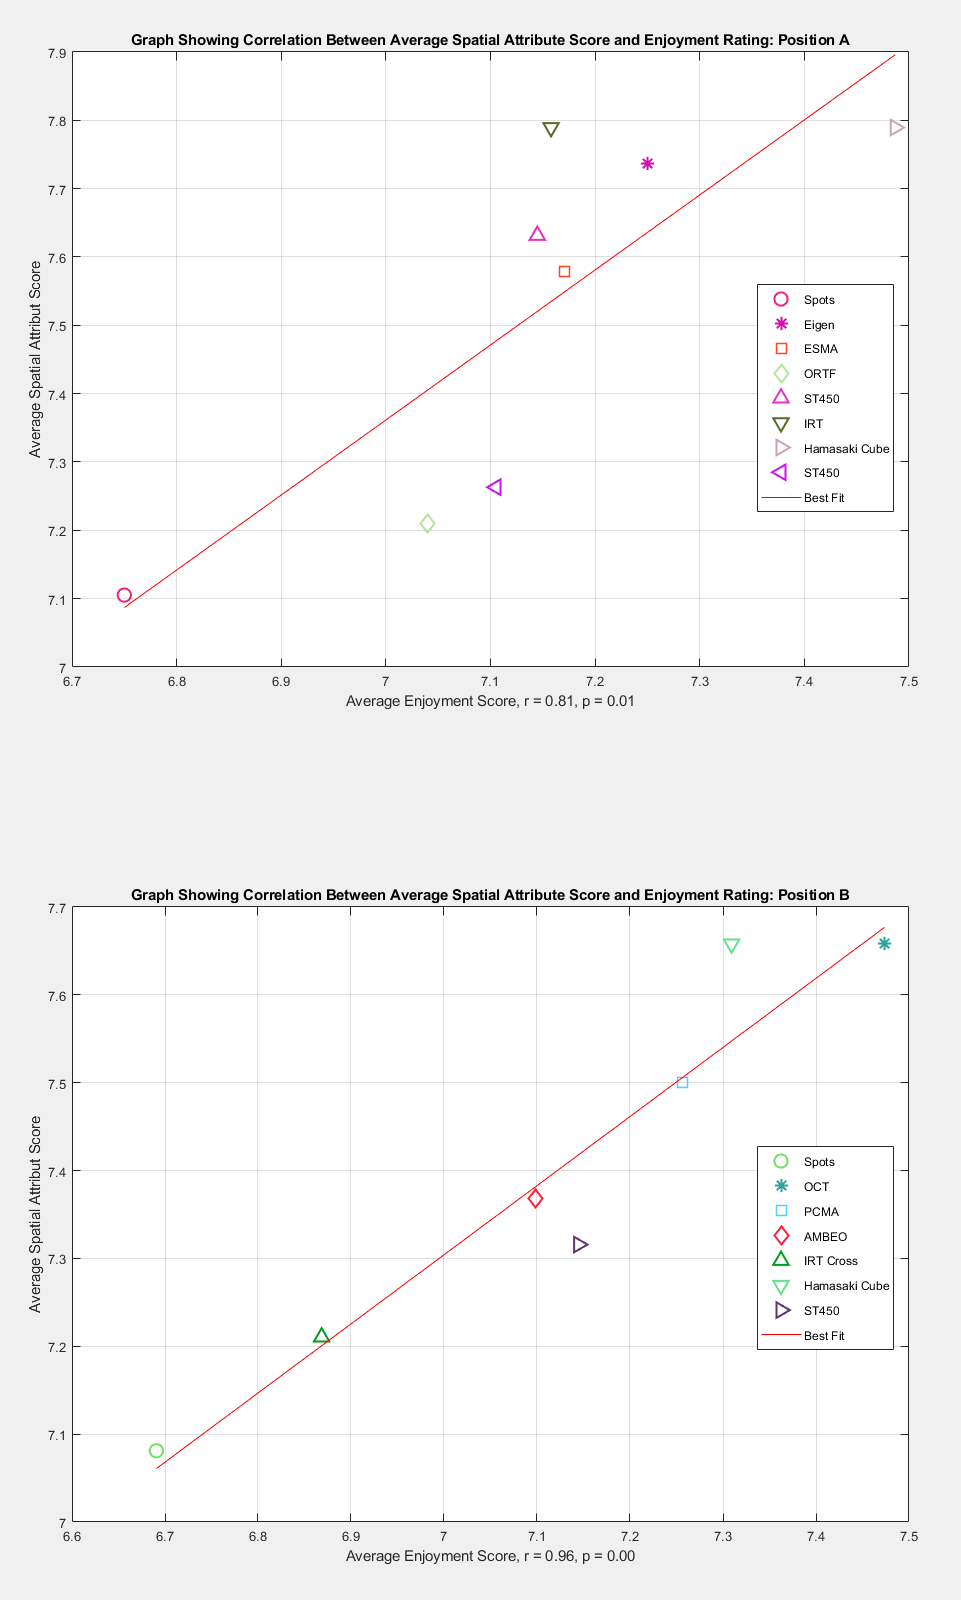
\includegraphics[width=0.5\textwidth]{images/stats/enjoyment_corr_V1.PNG}
		\caption{Two graphs showing a positive correlation between enjoyment rating and spatial attribute scores for viewing positions A (Top) and B (Bottom).}
		\label{image:enjoyment} 
	\end{figure}		
